\documentclass{sty/IOS-Book-Article}

\usepackage{mathptmx}
\usepackage{graphicx}
\usepackage{array}
\usepackage{amsmath}
\usepackage{amssymb}
\usepackage{csquotes}
\usepackage{multirow}
\usepackage{booktabs}
\usepackage{subcaption}
\usepackage{microtype}
\usepackage{todonotes}

\begin{document}

\begin{frontmatter}
  \title{How to Adapt LLMs for Free-Text Medical Event Processing}
  \runningtitle{How to Adapt LLMs for Free-Text Medical Event Processing}

  \author[A]{\fnms{Mart-Mihkel} \snm{Aun} \thanks{Corresponding
      Author: Mart-Mihkel Aun, Institute of Computer Science, University
  of Tartu, Estonia; E-mail: mart-mihkel.aun@ut.ee.}}
  \author[A]{\fnms{Maria} \snm{Malk}}
  \author[A,B]{\fnms{Sulev} \snm{Reisberg}}
  \author[A]{\fnms{Kerli} \snm{Mooses}}
  \author[A,B]{\fnms{Jaak} \snm{Vilo}}
  \author[A]{\fnms{Raivo} \snm{Kolde}}
  \author[A]{\fnms{Sven} \snm{Laur}}

  \runningauthor{M.-M. Aun et al.}
  \address[A]{Institute of Computer Science, University of Tartu, Estonia}
  \address[B]{STACC, Estonia}

  \begin{abstract}
    Large language models can be used to extract candidate clinical
events from free-text electronic health records, but their outputs
require validation. Such a manual review produces labelled examples
that can subsequently be used to improve model performance. We
compare few-shot prompting, fine-tuning, and prompt tuning for
context-aware phrase classification, focusing on the identification
of drug discontinuation events in Estonian clinical notes. To gain
insights, we first examine how performance scales with training-set
size on a well-established public benchmark. We then validate the
methods on manually annotated candidate events from the Est-Health 30
dataset. We show that, in a low-data setting, prompt tuning matches
or outperforms full fine-tuning for instruction-tuned models while
training up to 10,000 times fewer parameters. These findings suggest
that soft prompts can effectively use limited clinical annotations
while requiring far fewer trainable parameters, although their
effectiveness depends on the underlying model.

  \end{abstract}

  \begin{keyword}
    prompt tuning\sep phrase classification\sep clinical natural
    language processing\sep Estonian\sep parameter-efficient fine-tuning
  \end{keyword}
\end{frontmatter}

\section{Introduction}

Most medical studies rely on structured data, which often lacks
important clinical details~\cite{kho2011,Seinen2025}. For Estonian
data, free-text clinical notes have enabled the extraction of adverse
drug events for pharmacogenetic research~\cite{sarg2025} and detailed
descriptions of drug discontinuation
events~\cite{suvalov-2026-extract}. Both studies used large language
models (LLMs) for limited-scope extraction of information related to
specific medication groups. In contrast, we investigate whether LLMs
can be applied to the entire free-text EHR corpus without relying on
structured data to preselect or filter relevant records. Our
experiments are conducted on a large-scale real-world clinical
dataset, Est-Health~30~\cite{reisberg2026eh30}.

In this study, we extend the work of \v{S}uvalov \emph{et
al.}~\cite{suvalov-2026-extract} by creating a heterogeneous dataset
of drug discontinuation events and by assessing the number of
annotations required to train different LLM-based methods. As manual
prompt engineering with carefully selected few-shot examples is often
brittle and sensitive to wording~\cite{brown2020language,liu2024gpt},
we try alternatives. Fine-tuning can improve performance, but may
suffer from catastrophic forgetting when only a few hundred
annotations are available. Also, the resulting models are often
gigabytes in size. Prompt tuning offers a lightweight alternative and
has been shown to improve performance in multilingual transfer on
low-resource languages
\cite{philippy-etal-2024-soft,lester2021power}. Moreover, the
resulting soft prompts are interpretable and only a few kilobytes in
size, making them easy to share and publish with minimal privacy risk.

\section{Methods}

Information extraction typically consists of two stages: identifying
candidate phrases and determining their meaning through
classification. In this study, we focus on the phrase classification
task and study how different adaptations of LLMs cope with it.

\subsection{Model Benchmarking and Data Scaling}

Fair evaluation of LLM-based methods in this context is challenging.
Meaningful and reproducible evaluation requires a large, consistently
annotated public dataset. Because such medical datasets are rarely
available, we first evaluate model families on a well-established
non-medical benchmark dataset
MultiNERD~\cite{tedeschi-navigli-2022-multinerd} to understand
general properties and trends. This dataset contains named entity
annotations for Wikipedia and Wikinews sentences. Its diverse
annotation scheme includes 16 entity classes across more than 160,000
sentences, providing substantial variability for model evaluation.
Our main interest is how performance scales with the amount of
annotated training data and which adaptation method performs best
when ample training data are available. We report performance using
the F1 score, which balances precision and recall.

\subsection{Creation of the Target Clinical Dataset}

Following \v{S}uvalov \emph{et al.}, we consider only patient
anamnesis notes. We use MedGemma with system prompts adapted from
\cite{suvalov-2026-extract} to extract candidate drug discontinuation
events for manual review. Although originally designed for a narrower
extraction task, these prompts achieved over 90\% recall, making them
suitable for candidate generation.

The event cohort was assembled from Est-Health 30, which contains
centrally collected electronic health records from 2012--2024 for a
random 30\% sample of the Estonian
population~\cite{reisberg2026eh30}. To capture rare drug
discontinuation events, we selected records based on drug purchases
and grouped them into four subcohorts: potentially incompatible drug
combinations, prolonged treatment gaps ($\geq$ 6 months), drug
discontinuations and switches. For each cohort, we collected all
anamnesis notes recorded within six months of the index event. After
phrase extraction with MedGemma (27B), we randomly sampled 1,000
potential discontinuation phrases from each cohort, yielding a
dataset of 4,000 notes. Three experts annotated 3,300 candidate
phrases. Each anamnesis note was annotated with one or more event
labels. The labels \emph{adverse reaction}, \emph{treatment success},
\emph{treatment inefficacy}, \emph{contraindication or unsafe co-use}
and \emph{other} represent reasons for drug discontinuation, whereas
\emph{adverse reaction without discontinuation}, \emph{dosage change}
and \emph{other non-discontinuation} describe medication-related
phrases without discontinuation. Unsuitable phrases were labelled
\emph{incorrect phrase}.

\subsection{Experimental Setup and Performance Metrics}

For the MultiNERD benchmark, we evaluated model performance using
training sets of 10, 100, 1,000 and 20,000 labelled examples. For the
clinical dataset, we repeated the analysis with training-set sizes
ranging from 100 to 2,500 annotations. In all experiments, the test
set remained fixed. For the clinical task, we also collapsed the nine
event labels into a binary outcome indicating a drug discontinuation event.

The main experimental factors were model family and size, learning
method, training-set size, and prompt initialisation. For prompt
tuning, we compared how random initialisation compares with a
user-selected starting prompt describing the task. We recorded test
F1, predictions, model checkpoints, and learned prompt embeddings.

Experiments were run on a single GPU using BF16 precision and 8-bit
AdamW optimiser. We used a batch size of 8 and trained models with
early stopping based on validation F1, using learning rates of $5
\times 10^{-5}$ for fine-tuning and $10^{-2}$/$10^{-3}$ for prompt
tuning of decoder/encoder models.

\subsection{Context-Aware Phrase Classification}

The objective of context-aware phrase classification is to assign a
binary or multiclass label to a candidate phrase using both the
surrounding text and task instructions (\emph{prompt}). Annotated
examples are used to further adapt the model to the target
classification task. For autoregressive LLMs, context-aware
classification can be framed as a question-answering task in which
the model's output represents the target class. For encoder models
such as \textsc{BERT}, the task must be reduced to standard text
classification. The prompt and context can be encoded as part of the
input sequence using \textsc{[sep]} tokens for explicit structuring.
The output is passed to a linear classification head.

Prompting itself can be done by asking questions in natural language.
Supervised learning allows us to move beyond manual prompt
engineering. Parameter-efficient fine-tuning (PEFT) updates only a
small subset of model parameters. For example prompt tuning learns a
virtual (\emph{soft}) prompt prepended to the input, leaving the base
model unchanged~\cite{lester2021power}.

\section{Results}

\subsection{General Scaling laws}

To identify promising models for prompt tuning, we first benchmarked
different model families on a 20,000-sample training set from
MultiNERD. Results are shown in Table~\ref{tab:multinerd}. For all
models, fine-tuning and prompt tuning substantially outperformed the
few-shot baseline. For most model families, the two approaches
achieved comparable performance. Differences between random and
informed prompt initialisation were small.

\begin{table}[ht]
  \centering
  \footnotesize
  \setlength{\tabcolsep}{4pt}
  \renewcommand{\arraystretch}{0.9}
  \caption{
    MultiNERD test Macro-F1 (\%), trainable parameters, and virtual
    prompt length after three epochs on 20,000 English sentences. FT
    = fine-tuning; PT = prompt tuning (pre. = system-prompt
    initialisation, rand. = random initialisation); FS/head =
    five-shot prompting for decoders or an encoder classification
    head. %Bold indicates the highest F1 in each column.
  }
  \label{tab:multinerd}
  \begin{tabular}{lrrrrrrrr}
    \toprule
    Model     & Instructable & Params & PT params & FT          & PT (pre.)   & PT (rand.)  & FS/head & Prompt tokens \\
    \midrule
    mmBERT    & No           & 307M   & 23K       & \textbf{91} & 88          & 73          & 14      & 15 \\
    Gemma 3   & Yes          & 4.3B   & 145K      & \textbf{86} & 73          & 74          & 43      & 57 \\
    Llama 3.1 & Yes          & 8B     & 237K      & 81          & \textbf{88} & 79          & 52      & 58 \\
    Qwen 3.5  & Yes          & 9B     & 241K      & \textbf{84} & 83          & \textbf{84} & 64      & 59 \\
    \bottomrule
  \end{tabular}
\end{table}

Figure~\ref{fig:multinerd-scaling} shows how performance changes with
the number of available training samples. F1 score generally improves
with increasing training-set size. Prompt tuning tends to perform
better with limited training data, whereas fine-tuning can surpass it
as the dataset grows. Across all models, 1,000 training examples were
sufficient to reach near-optimal performance, with only modest
improvements thereafter.

\begin{figure}[ht]
  \centering
  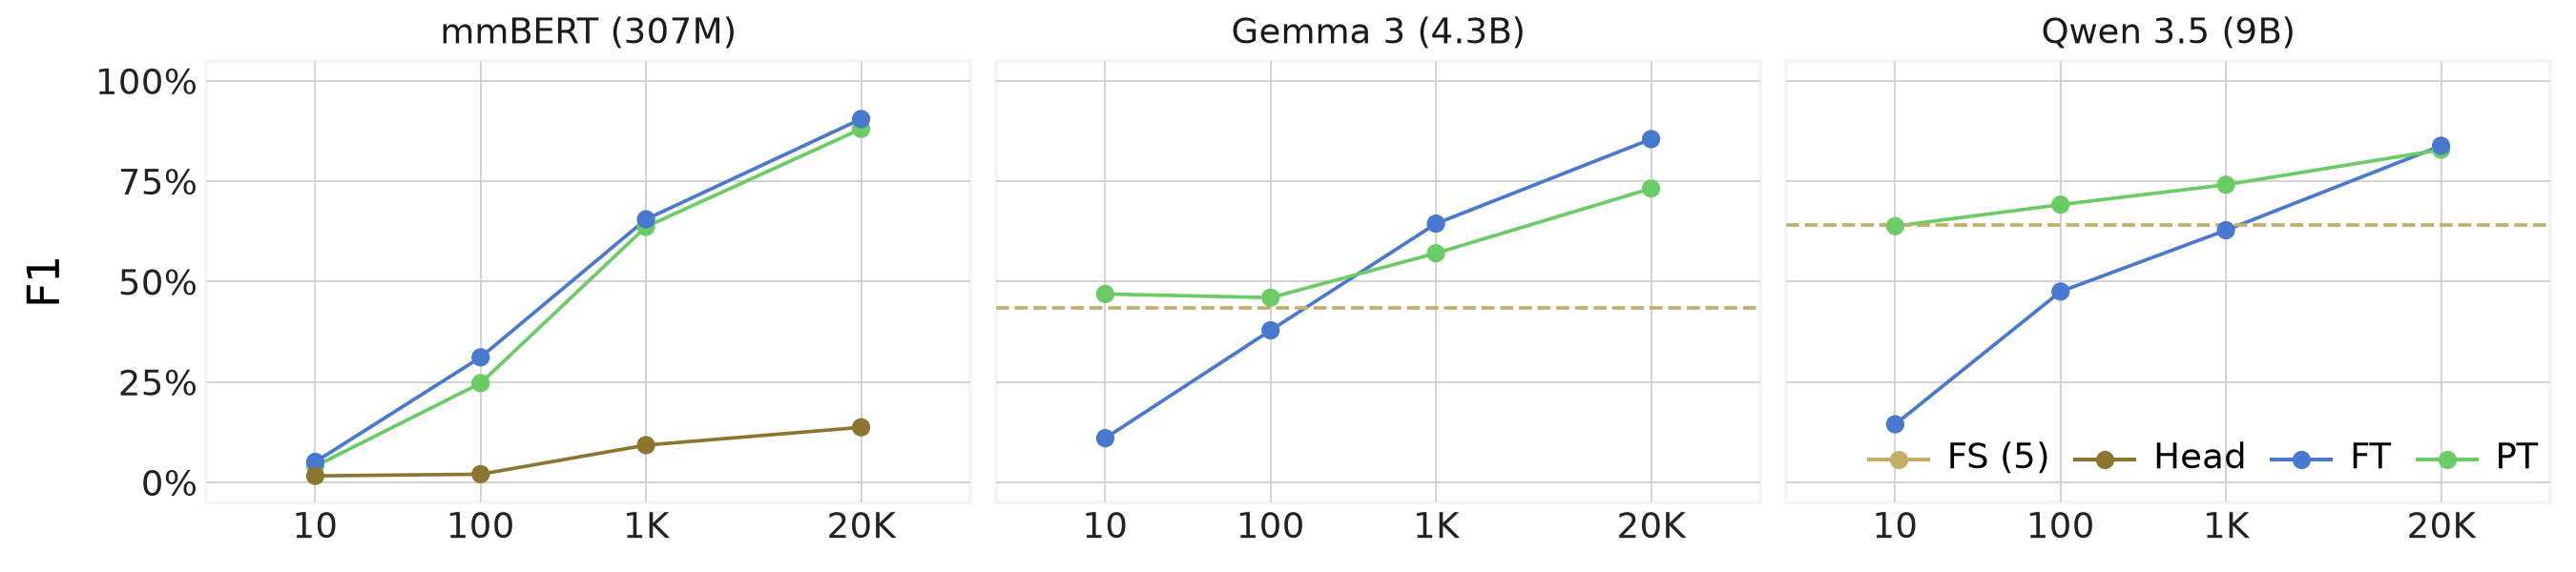
\includegraphics[width=\textwidth]{fig/multinerd-data-scaling.png}
  \caption{
    MultiNERD test Macro-F1 (\%) by number of labelled training
    sentences. FT = fine-tuning; PT = prompt tuning; Head = encoder
    classification head and FS (5) = five-shot prompting as baselines.
  }
  \label{fig:multinerd-scaling}
\end{figure}

\subsection{Performance on Drug Discontinuation Data}

Figure~\ref{fig:eh30-scaling} shows how performance changes with the
number of annotated phrases. Prompt tuning did not outperform the
baseline for mmBERT, possibly due to limited capacity for instruction
following in the Estonian medical domain. In contrast, it clearly
outperformed fine-tuning for the other two models. Occasional drops
in performance likely reflect statistical instability, as the smaller
training sets provide insufficient data to offset the effects of
unrepresentative samples.

\begin{figure}[ht]
  \centering
  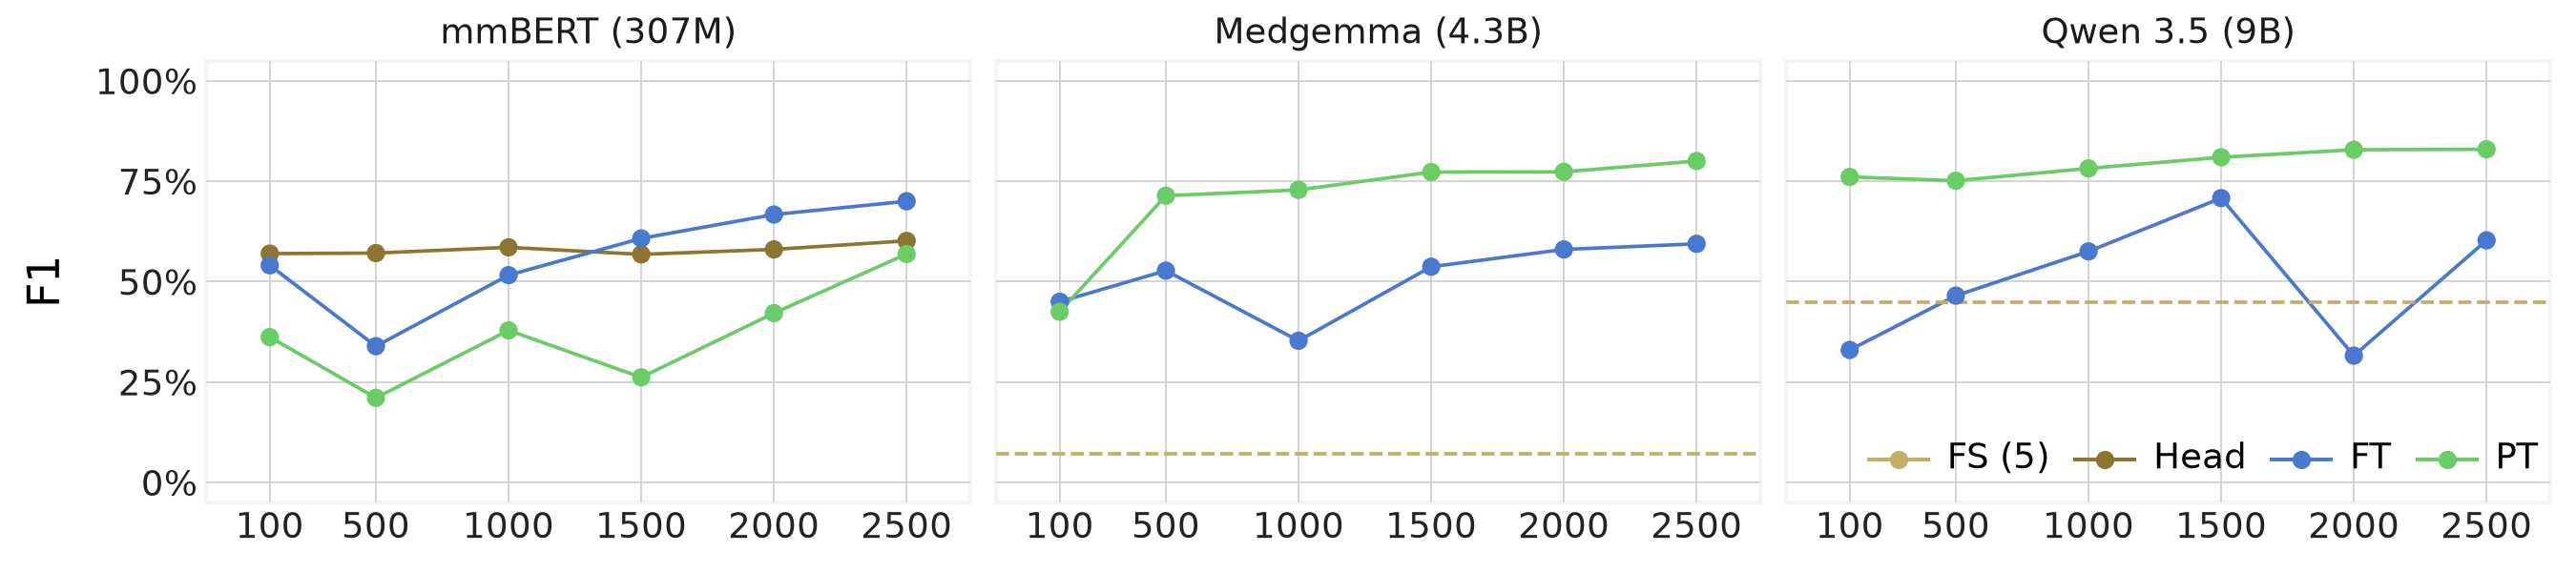
\includegraphics[width=\textwidth]{fig/eh30-data-scaling.png}
  \caption{
    Estonian medication-discontinuation test F1 (\%) by training-set
    size, measured as the number of labelled anamnesis notes and
    evaluated on a fixed test split. FT = fine-tuning; PT = prompt
    tuning; Head = encoder classification head; FS (5) = five-shot
    prompting, shown as a fixed decoder baseline.
  }
  \label{fig:eh30-scaling}
\end{figure}

\section{Discussion}

The main limitation of our study is its scope. Ideally, model
performance should be evaluated across a broader range of medical
tasks and datasets. This would help determine whether the weaker
performance of mmBERT was a fluke or reflects a more general
limitation on complex clinical classification problems. A second
limitation is dataset size -- the number of annotated examples was
insufficient to detect saturation.

\section{Conclusions}

Results suggest that prompt tuning is a strong alternative to
fine-tuning in low-data setting. Another benefit is model size --
prompt tuning trains three to four orders of magnitude fewer
parameters and produces artefacts measured in kilobytes. This makes
prompt-tuned models easier to publish, as they pose a lower risk of
privacy leakages. Soft prompts can also be translated back into
natural language for further inspection.

\section{Acknowledgements}

This work was funded by the Estonian Research Council (PRG1844); the
European Union and the Estonian Ministry of Education and Research
(TEM-TA72); the European Union’s Horizon Europe research and
innovation programme and the Estonian Ministry of Education and
Research through grant agreements No. 101060011 (TeamPerMed),
101057639 (SafePolyMed) and 2021-2027.1.01.24-0444; and the Estonian
Ministry of Education and Research (TK213) EXAI.


\bibliographystyle{sty/vancouver}
\bibliography{ref}

\end{document}
